\documentclass{article} % For LaTeX2e
\usepackage{hyperref}
\usepackage{url}
\usepackage{times}
\usepackage{bbm}
\usepackage{amsmath, amssymb,, epsfig}
\usepackage{sectsty}
\usepackage{pdfpages}
\usepackage{indentfirst}
\usepackage{graphicx}
\usepackage[margin=1in]{geometry}
\usepackage{times}
\usepackage{bbm}
\usepackage{amsmath, amssymb,, epsfig}
\newcommand*{\QEDA}{\hfill\ensuremath{\blacksquare}}
\usepackage{sectsty}
\usepackage{pdfpages}
\usepackage{indentfirst}
\usepackage{graphicx}
\usepackage[margin=1in]{geometry}

\title{NBA Predictions}

\author{Lee Richardson (lrichard) \\ Daren Wang (darenw) \\ Chi Zhang (chiz2) \\ Xiaofeng Yu (xiaofen1)}  

\newcommand{\fix}{\marginpar{FIX}}
\newcommand{\new}{\marginpar{NEW}}

\begin{document}

\maketitle

\begin{abstract}
Last season, the defending champion Miami Heat lost back to back games against the lowly Detroit Pistons and Milwaukee Bucks. While a two game stretch like this is certainly unlikely, it exemplifies the impact randomness has on basketball games. In this paper, we look at various predictions made regarding National Basketball Association (NBA) basketball games. Specifically, we see that we can predict the outcome of single games with a maximum of around 70\% using various Machine Learing algorithms. We use these predictions to simulate the outcome of the 2012 and 2013 season, and our predictions landed us in the top 15 of all publically available NBA projection systems in both years \cite{projections}. Finally, we saw that the recently developed Regularized Adjusted Plus Minus (RAPM) statistic was a better predictor than any other statistic in our database. 
\end{abstract}

\section{Introduction}
	In recent years, there has been lots of talk in NBA circles regarding the rise of statistical analysis\cite{revolution}. This has been in the works for years, most notably starting with Dean Oliver's Basketball on Paper, which was the cornerstone of basketball statistics for years. More recently, new data has become available, most notably from play by play events as opposed to box score statistics. There is also data from camera's which track player's motion, but this is mainly proprietary, with few exceptions. \\

	In this paper, we look to harness all of the data publically available to predict the outcome of NBA basketball games. In section two, we will look at previous attempts at this problem as well as more recent data we could use for predictions. Next, we will describe how we obtained and put together our dataset, and give information on how one could access it. In section four, we describe our efforts of predicting games using different algorithms, features, and model selection techniques. Then we will discuss how we used our game predictions to obtain a distribution of for each teams record, and compare this with other projection systems. Finally, we will end with a discussion of what we learned and ways to improve our predictions. 

\section{Related Works}
	%%% TALK ABOUT NBA ORACLE AND DATA MINING TO COMPARE PREDICTION ACCURACIES
	We looked into the literature to see if anyone had worked on the same or similar problems. We found a few papers, specifically \cite{nba_oracle} and \cite{data_mining}, which also attempted to predict the results of NBA games. These papers used linear regression, logistic regression, naive bayes, and SVM's to predict the outcome of single games. They also used the same loss function that we are proposing, which gives us a prediction rate to shoot for when implementing our algorithms. Specifically, \cite{nba_oracle} achieved the highest single season classification rate of 73\% in the 1996 season using linear regression. All of the other seasons/algorithm combinations had error rates from the mid-high 60's to low 70's. \\

	%%% DELVE INTO THE RPM PAPER TO EXPLAIN WHY IT'S SO GOOD
	One advantage we believe we have compared with these groups is that we have a more robust feature set, most notably we have regularized adjusted plus minus (RAPM). RAPM has been anointed by many as the next big thing \cite{bigrpm} in the basketball statistics community, and we hope that using it as a feature can help differentiate our attempts at game classification. Taylor et al. have a great explanation of the statistic \cite{rpm}, but the basic idea is to split each game into miniature games, each one occurring in time periods when there's no substitutions. These ten players play a certain amount of possessions on offense and defense, and we can estimate their overall effect on both ends of the floor. RAPM adjusts for flaws in original plus minus, by correcting for the fact that player totals are heavily influenced by the play of his opponents and teammates, and by pooling information from previous seasons to reduce the margin of error. 


\section{Dataset}
\subsection{Challenges for dataset preparation}
Several challenges have to be handled for the dataset preparation phase.
\begin{itemize}
\item There are currently no ready-made data sources for our experiments. What we can find is several websites on NBA games. Since we are interested in statistics of thousands of games with hundreds of players, it's not realistic to acquire those data manually from websites.
\item Data sources from different websites have to be merged using a uniformed format. Different websites may treat player names and season matching differently. For example Roger Mason Jr. and Roger Mason are in fact same person from different websites, while uta and utah are different abbreviation for Utah Jazz.
\item Data needs to be stored in a proper manner so that our future experiments can be implemented based on a uniformed and easily accessible API.
\end{itemize}
To meet those challenges, we are writing our own web crawlers to get data from websites, then made lots efforts on ETL on ensure different data sources were properly matched and merged. Finally we stored all data into a SQLite database.
It's worth mentioning that we are making our dataset public online at \\
\url{https://github.com/leerichardson/game_simulation/blob/master/nba_rRegression_chi/nba.db}\\
Hopefully this will save some effort for anyone interested in research on NBA statistics recent years.\\

\begin{figure}
		\centering
		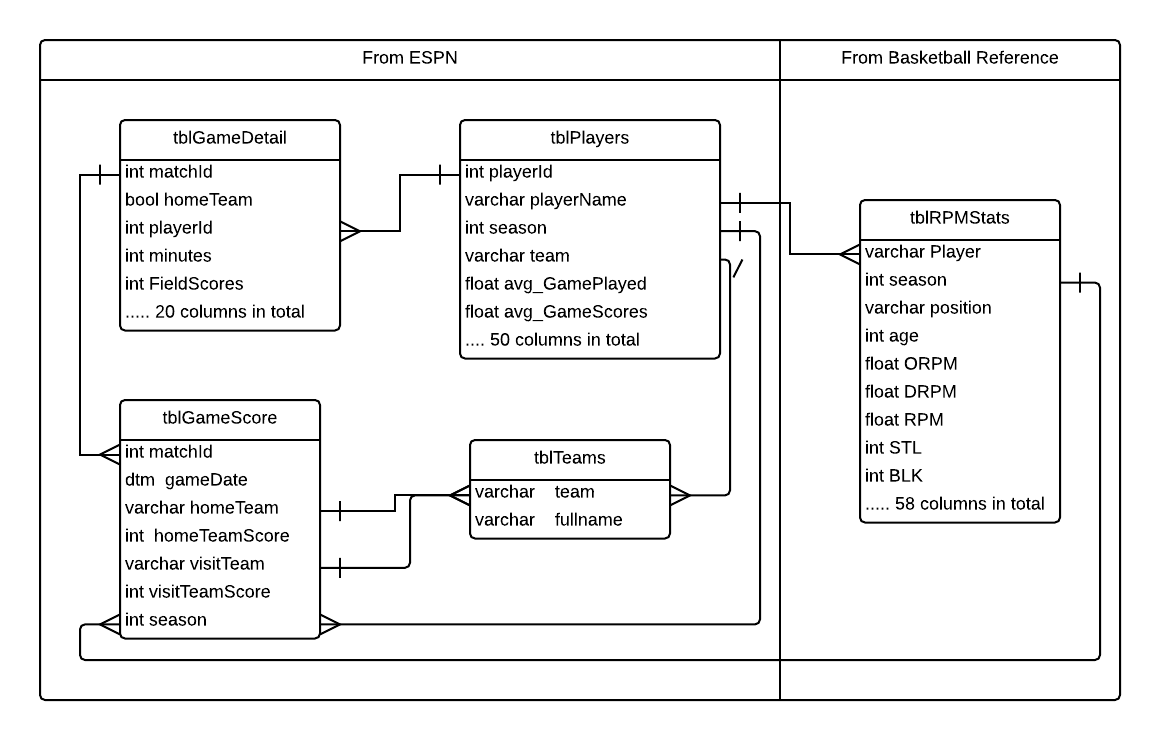
\includegraphics[width=150mm, height=120mm]{sqliteERDiagram.png}	
		\caption{Entity - Relationship graph for SQLite database. The database follows the third normal form to ensure there is no redundancy. Two main data sources of the dataset are ESPN and Basketball References websites. Lines between tables indicate the primary key - foreign key relationship between dataset entities.}
		\label{fig:database}
\end{figure}

\subsection{Data Sources}
	We did not have a processed dataset for this project, so we created our own database. The three main sources we used were ESPN's NBA website \cite{espn}, basketball reference \cite{bball_ref}, and a new website from Jeremias Engleman \cite{rpm_data}. We used the ESPN data to get information about all NBA games from 2009-2014. Specifically, this includes the game score, the home and away teams, the players involved and their individual statistics. Also from ESPN, we have a player database, which has 50 individual statistics for each player in each season. There are 7139 games in this dataset. \\

	The next data source we used was basketball reference \cite{bball_ref}. The main reason we used this site is because they have a larger individual player database, with information dating back to the 1950's and more advanced statistics, such as the widely used Player Efficiency Rating (PER), compared with the box score stats provided by ESPN. \\

	The final source we used was from a website put together by Jeremias Engleman \cite{rpm_data}. This site has RAPM statistics dating back to the 1980's. This statistic has been widely adopted in the NBA statistics community, and it's one of the few trustworthy stats which provides an individual assessment of defense. As we see below, RAPM is a very useful feature in predicting game outcomes. \\

	%%% WEB CRAWLERS
\subsection{Web Crawlers}
	To obtain all of these datasets, we used webcrawlers to pull them off their websites. All of these scripts can be found in our Github repository \cite{gitrepo}. For the ESPN data, we used the BeautifulSoup package in the Python language. For the other two datasets, we used the XML package in R. \\

	%%% TALK ABOUT MERGING SOURCES 
	\subsection{Merging Sources into One Database}
	One of the major obstacles in our project has been combining these three data sources into one single database. The ESPN dataset had both match and playerID's for each game, so merging the game statistics with the ESPN player database wasn't very difficult. However, the basketball reference and RAPM dataset didn't have these identifiers, so it was more challenging to put them together. We ended up using the player's name, team, and season to join both of these datasets together with ESPN. Some common problems we had were inconsistent spelling of names in different datasets, inconsistent team names, teams have changed cities, etc.. In the end, we were able to sync most of the idiosyncracies between the three datasets, which is important because we will have more interesting features than just box score statistics. That being said, we don't doubt that there will still be further cleaning to do, and we will deal with these situations as they arise. \\

\section{Experiments}
	%%% TWOFEATURE MATRICES/.. LARGE AND JUST RPM/PER
	\subsection{Training and test datasets}
	We have put a substantial amount of time into constructing our training and test datasets. The dataset consists of both RAPM data and ESPN's player basic statistics(i.e, average points or rebounds of a season). To create the dataset, we went through each match to find the players on each team, and merged these players statistics from the previous season with the match results in the current season. We then sum up the players statistics to form home team and away team statistics.   To form the RAPM features, we used each players average minutes pergame from the season before as weights to compute weighted offensive and defensive RAPM statistic for each team. Say there's n players on each team, each playing m minutes per game with and RAPM score r in the previous season. Then the formula for the players weights and team offensive RAPM is:

	\begin{align*}
		w_i &= \frac{m_i}{\frac{1}{n}\sum_{i=1}^{n} m_i} \\
		\text{Team Offensive RAPM} &= \frac{1}{n}\sum_{i=1}^{n} w_i \times r_i 
	\end{align*}

	%%% TABLE OF EXAMPLE MATRIX %%%
	\begin{table}[ht]
	\centering
	\begin{tabular}{rrrrrr}
	  \hline
		ORPM\_home & DRPM\_home & ORPM\_away & DRPM\_away & homeWin \\ 
	  \hline
		-0.28 & 0.89 & 0.65 & 0.18 & 1 \\ 
	  	-0.28 & 0.89 & 1.15 & 1.05 & 1 \\ 
	  	-0.29 & 0.99 & -1.44 & 0.12 & 1 \\ 
	  	 0.03 & -0.66 & 0.04 & 1.09 & 1 \\ 
	  	 0.28 & 1.26 & -0.81 & -0.20 & 0 \\ 
	  	-0.75 & -0.46 & 0.51 & 1.02 & 1 \\ 
	   \hline
	\end{tabular}
	\caption{A look at what our training and test datasets look like. The first four columns are features and the 5th column (indicating whether or not the home team won the game) is our label.}
	\label{table:matrix}
	\end{table}
Before training the model, we would like to get a general feeling about how are the features related to the game results
In figure \ref{feats}, the left is a plot showing the correlation between home team RPM and visit team RPM in our dataset. This shows that our data is not linearly separable for these two features, which is common among this dataset. However, the green dots(corresponding to home team loss) are more likely to accumulate on the lower right and the red ones are on the top left corner of the plot. A classification boundary like  the diagonal line in the plots shows that it will classified a majority of the data set and making fewer mistakes.  Also, we do see that there is some signal between wins and losses for these two features, as a higher score indicated a higher chance of winning the game. On the right, we look at team RAPM in wins compared with losses. As we can see, RAPM is clearly higher in wins than losses, so their is clear signals coming from this feature, as expected.


\begin{figure}[h]
	\centerline{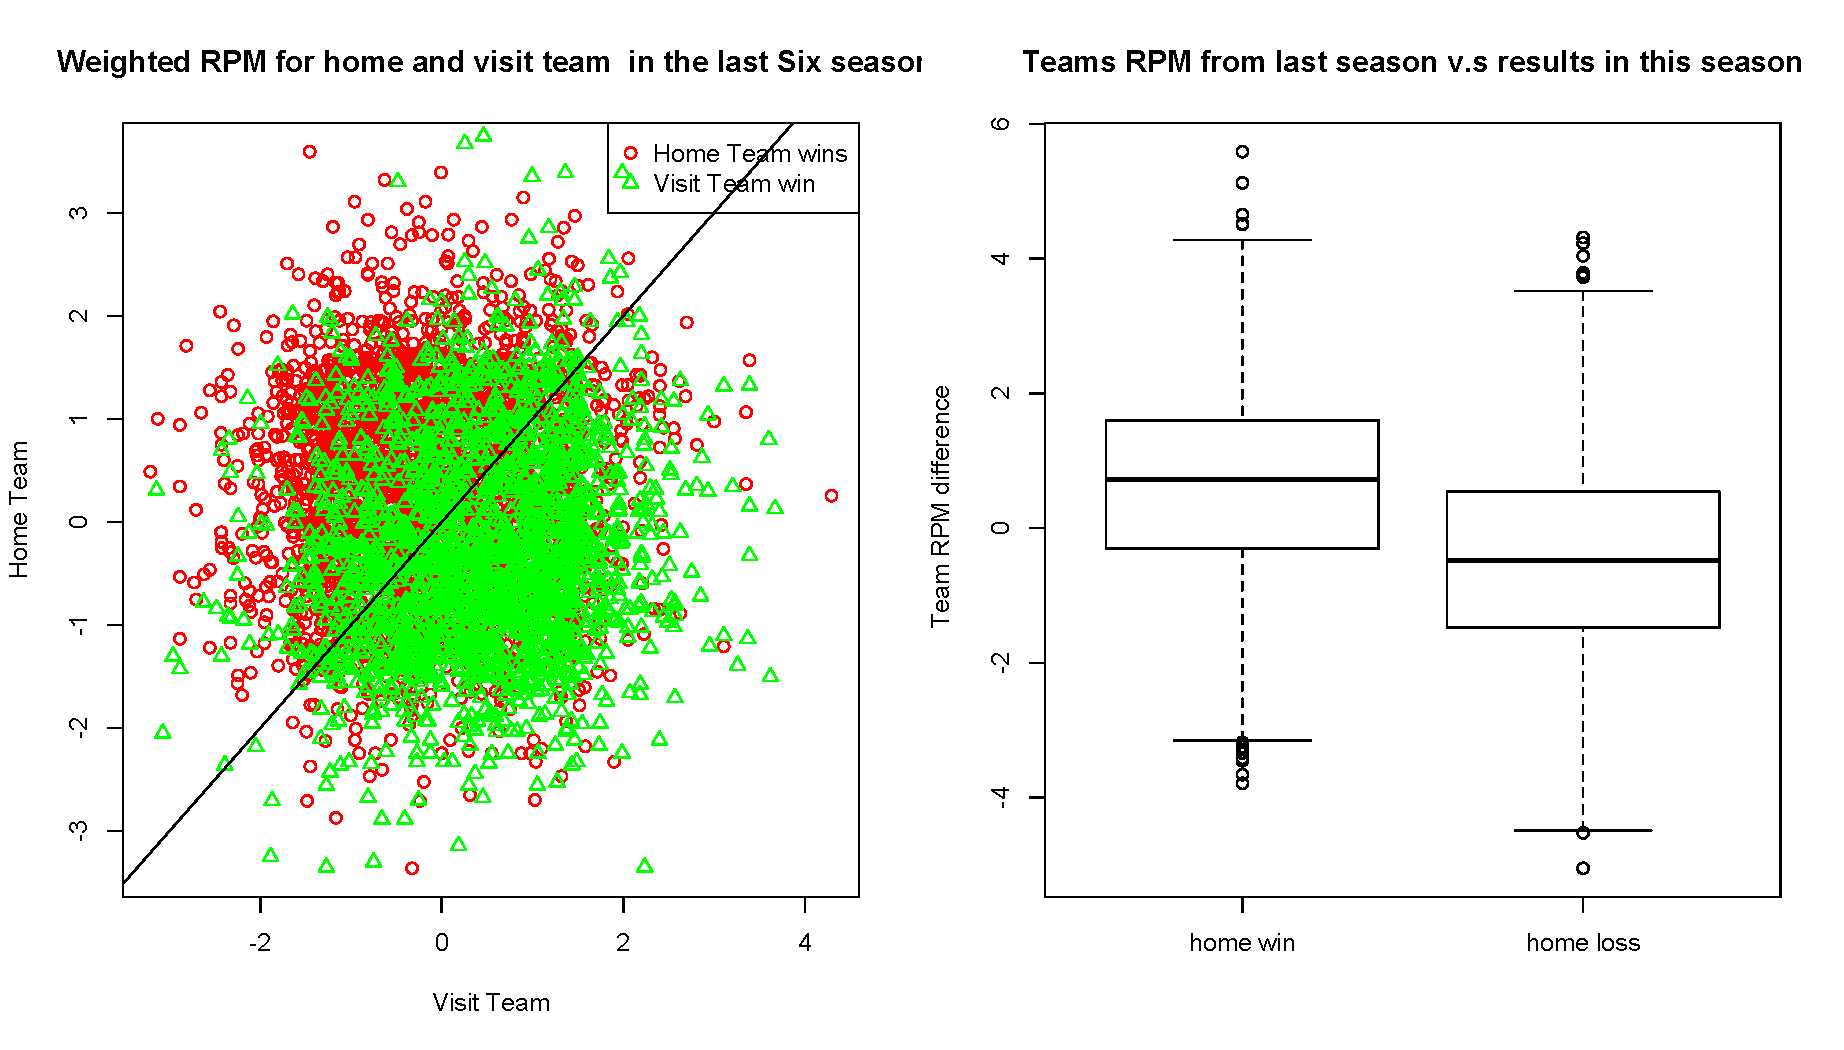
\epsfig{file=features.pdf, width=7in,height=3.25in}}
	\caption{Left: visit team  RPM against home team RPM with green dots meaning visit team wins and red dot meaning home team win. Right: A box plot of RPM. Y-axis represent the the RPM difference between home team and visit team. }
	\label{feats}
	\end{figure} 
	
	
	\subsection{Training the model and the test error}
	The data set is now ready. We have in total 6 season data. We first would like to try different model on our data set. For each model we try, we will split our data set into training part and testing part. For example if we try to predict the results in season 2010, we will train the model using  season 2008 and 2009 data.�We then use our trained model to predict the results of season 2010. %Chi's plot pleas
	
	\begin{figure}
		\centerline{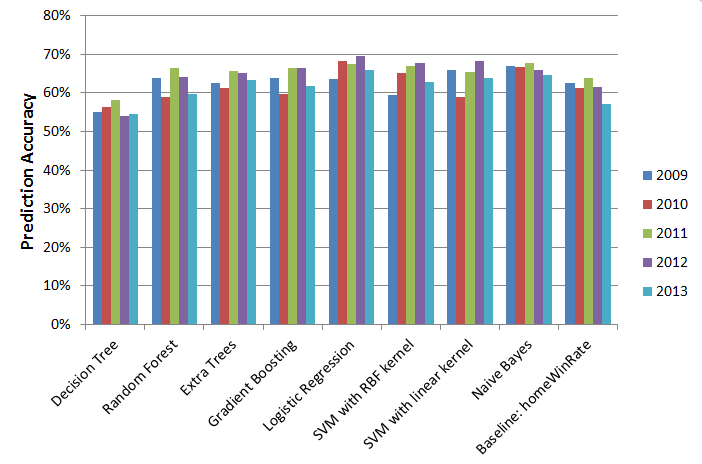
\epsfig{file=algorithms.png, width=5.5in,height=3.50in}}
		\caption{This plot shows the test error for our different algorithms in all of our years. From this, we see that Naive Bayes and Logistic Regression gave us the best overall test error. For each testing year, we used all the previous years as training data.}
		\label{fig:database}
\end{figure}
	
	
	Figure  \ref{fig:database} demonstrates the test error of different model. It turns out that the Naive Bays and linear model have the best testing accuracy.  Note that based on the observation we make in the last section, we believe that simple model (with linear classification boundary) will have good performance. The test accuracy plot agrees with our intuition.\\ \\
	Notice so far we have 44 features in each of our model. Thus we believe that feature selection will help us to improve the prediction accuracy. Here we will illustrate our feature selection using linear regression. For other models the idea would be similar. For linear model, we try lasso and AIC to accomplish the feature selection. For lasso, we choose $\lambda$ 
, the degrees of freedom, to minimize  the CV, and then fit the model using that $\lambda$. For AIC, we use set our minimal and full model, and then perform  stepwise AIC feature selection. 	
		\begin{table}[ht]
	\centering
	\begin{tabular}{rrrrrr}
	  \hline
		 & Full model (linear) & & Lasso & & AIC \\ 
	  \hline
		2009 & 0.6544715 && 0.6658537 && 0.6617886  \\ 
	  	2010 &0.6739837  &&0.6853659 &&0.6788618    \\ 
	  	2011 & 0.6676768 & &  0.6626263 &&  0.6717172  \\ 
	  	2012 &0.6786005& & 0.6712775 && 0.6818552  \\ 
	  	2013 & 0.6601626 && 0.6634146 && 0.6601626  \\ 

	   \hline
	\end{tabular}
	\caption{A look at how feature selection change the prediction accuracy.}
	\label{table:matrix}
	\end{table}
	
	It turns out that AIC in general helps to find a more predictive model.  Note that the absolute increment is not significant in this case. However, as discussed later in the paper, the best prediction accuracy in the market is around 70$\%$, while if one always predict home team win, the accuracy is around 60$\%$.  Take this into consideration, the improvement from AIC is not negligible.
	
\section{Simulation}	

\begin{figure}
  \centering
  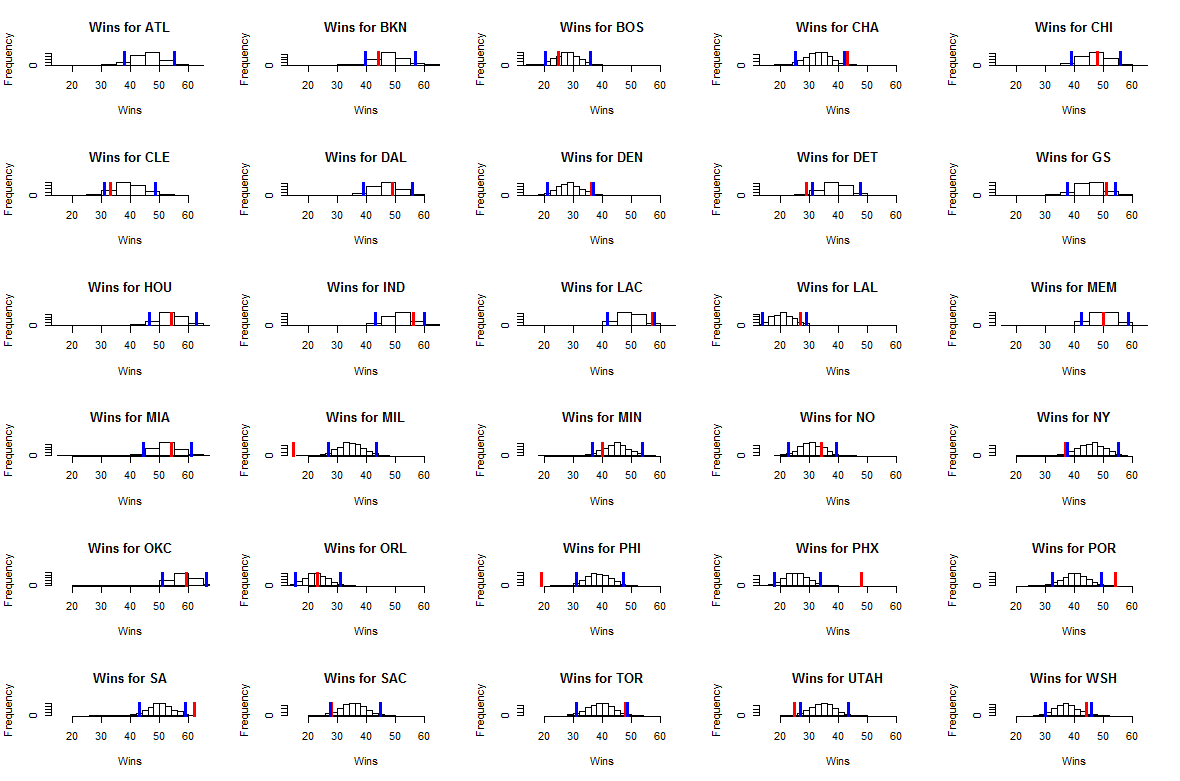
\includegraphics[height=15cm, width=15cm]{season_wins.png}
  \caption{Results from simulating the 2013 NBA season 1000 times, using probabilities from our best Logistic regression model. The blue lines represent our confidence intervals whereas the Red lines represent the actual number of wins for each team. Our simulations trapped the true number of wins in 70 \% of our intervals.}
  \label{fig:simulations}
\end{figure}

In order for the various classifier's to predict which team would win each game, they generate probabilities for each team, and predict the maximum. Another natural way to utilize these probabilities is to use them to simulation the entire season. Specifically, by generating Uniform(0,1) random variables, and scaling the probabilities to sum to one (when necesary), we were able to stochastically determine the outcome of each game, and simulation each season to see the distribution predicted win totals for each team. Figure \ref{fig:simulations} shows the win distributions for each team, using logistic regression for the 2013-14 season. Out of the two best classifiers (Naive Bayes and Logistic Regression), logistic regression performed much better in the two seasons we simulation, using both the Root Mean Squared Error (RMSE) and Median Absolute Deviation (MAE) loss functions. This is because the Naive Bayes prediction outcomes were much more extreme than logistic regression. For example, the standard deviations of the number of wins predicted for each team using Naive Bayes were 16.12 and 17.07, compared with 9.66 and 9.68 for logistic regression. Due to computing and time restrictions, we weren't able to run as many simulations as originally intended. However, we did run 1000 2013 simulations various times, and the win distribution was nearly identical, meaning that 1000 is a safe range for convergence. \\

Predicting the number of wins for each team preceding each season is a much more popular task than computing test errors, so we were able to compare our projections to other systems using the RMSE loss function (which is the loss function used by others \cite{projections}). Our RMSE for 2012 was 7.54 and 9.7278 in 2013. This would be in the top 20 for the past two seasons. Had we used Naive Bayes as opposed to Logistic regression, our system would have consistently 


\section {Conclusion}

%% General Theory for How to clasify. Why is predicting the outcomes of seasons harder?

%% Discuss why other systems bear us. (Projections, more developed, more nuances built in, etc...) Hollinger won, had been doing it the longers, mainly with PER

%% Why was 2013 so much less predictable than other years. Especially since we had the MOST training data. This gives some evidence to the theory that randomness may impact the results of these games more than a fancy classifier. sometimes the underdog will just win more. 

%% RAPM- Why did it do so much better? More information?? What does this say about SportsVU data's potential impact as a predictor?

%% Future developments: Using current season's data, Predicting the Spread, and building a projection of the RPM feature as opposed to just last year (more than one year, what to do with rookies? Etc..)


\begin{thebibliography}{1}

  \bibitem{nba_oracle} Matthew Beckler, Hongfei Wang, Michael Papamichael {\em NBA Oracle} 2009.

  \bibitem{data_mining} Dragan Miljkovic, Ljubiša Gajic, Aleksandar Kovacevic, Zora Konjovic {\em The Use of Data Mining for Basketball Matches Outcomes Prediction} 2010: SISY 2010

  \bibitem{rpm} Paul Fearnhead, Benjamin M. Taylor {\em On Estimating the Ability of NBA Players}. 2010: http://arxiv.org/pdf/1008.0705.pdf.

  \bibitem{bigrpm} Steve Illardi. {\em The next big thing: real plus minus}. 2014. ESPN.com

  \bibitem{rpm_data} Jeremias Engleman. http://stats-for-the-nba.appspot.com/

  \bibitem{bball_ref} Basketball Reference. http://www.basketball-reference.com/

  \bibitem{espn} ESPN. http://espn.go.com/nba/.

  \bibitem{gitrepo} Repository for Game Simulation. https://github.com/leerichardson/game\_simulation.

  \bibitem{projections} Weak Side Awareness Blog. http://weaksideawareness.wordpress.com/2013/04/23/checking-2012-13-nba-win-predictions-projections/

  \bibitem{revolution} Sam Hinkie and the Analytics Revolution in Basketball. NILKANTH PATEL http://www.newyorker.com/news/sporting-scene/sam-hinkie-and-the-analytics-revolution-in-basketball
  \end{thebibliography}

\end{document}